\documentclass[a4paper,15pt]{article}
\usepackage{graphicx}
\graphicspath{ {./images/} }
\begin{document}
     \begin{center}
     	Truss : An Overview
     \end{center}
    Truss is a structure consisting of organized objects in a shape of connecting triangles in such a way that it behaves as a single unit object. In order to enable the distribution of weight and grasp up the the fluctuating tension and compression without bending and shearing, it is made up of a web of triangles which is most stable form of geometry. In general, truss is used since it has a long life span and has least weight to the possible which in turn supports large loads and reduces deflections.\\
    
   Commonly used in bridges, roofs and high rise buildings, it gives high value for mega constructions like the Eiffel Tower, construction of a stadium and all. We can think of truss as a beam where the web consists of series of separate members instead of a continuous plate. In engineering perspective, a truss is a structure that comprises of one or more triangular units constructed in a linear pattern such that its ends are connected to joints which is called as external nodes. The external forces and reaction to the forces are considered to act only at the nodes and the results in forces in the members are either tensile or compressive forces. In truss, the lower horizontal structure and the upper horizontal structure carry tension and compression. The diagonal and vertical structure form the truss web and it carries shear stress. Technically, they are also in tension and compression where the exact arrangement of forces depends on the type of truss and on the direction of bending. The structures serves in order to stabilize each other in order to prevent buckling. The structures that are under compression are to be designed to be safe against buckling. After knowing the force on each member, we determine the cross sectional area of the individual truss members. The weight of truss structure depends directly on its cross section area. The effect of weight of individual structures in a large truss is generally insignificant compared to the force exerted by external loads.\\
   
   Later, after determining the minimum area of cross section of individual structures, it is dealt with bolted joints that involves shear stress of the bolt and connections used in the joints. The joints of truss can be designed as rigid, semi-rigid, or hinged.\\
   
   Equation of truss: \\
   
   The strain-displacement relationship is: \\
   \begin{eqnarray}
		   	\epsilon = \frac{du}{dx}\\
		   	\sigma = E\epsilon
   \end{eqnarray}

   From the law of equilibruim, we get,
   \begin{eqnarray}
   	A\sigma_x = T = constant
   \end{eqnarray}
   						
   Combining, the equations, we get:
   \begin{eqnarray}
   			AE\frac{du}{dx} = T = constant
   \end{eqnarray}
   						
   Differentiating with respect to x, we get,
   \begin{eqnarray}
   				\frac{d}{dx}(AE\frac{du}{dx}) = 0
   \end{eqnarray}
  						 is the equation of truss.
   
%   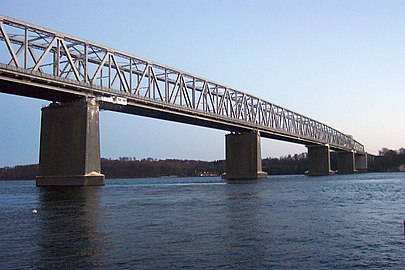
\includegraphics{3}\\
   Fig:  Truss in bridge\\
   
%   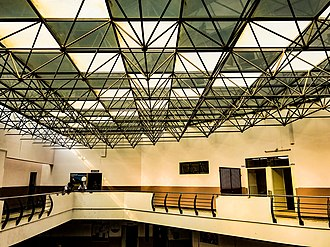
\includegraphics{2}\\
   Fig:  Truss in roofing\\
   
%   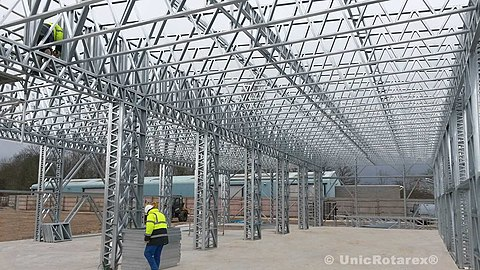
\includegraphics{5}\\
   Fig: Three Dimensional Truss\\
   
   
\end{document}